% The percent symbol creates a comment, which will be ignored by LaTeX when it creates your document.  They're useful for leaving yourself notes and organizing your work.
\documentclass{article}
\usepackage{amsmath, amssymb, tikz} % Required for math symbols
\usepackage[paper=letterpaper,
           hmargin={1in,1in},
           vmargin={1in,1in},
           ]{geometry}   % Allows you to change the margin sizes
\usepackage{enumitem}  % Required to re-label lists

\title{Homework 4}
\author{Xander} 
\date{Mar 3}

\begin{document}

\maketitle
%%%%%%%%%%%%%%%%% Don't delete anything above this line!

\section*{Exercise 14 4.2}  

Give an example of a graph that has exactly 7 different spanning trees. Note, it is acceptable for some or all of these spanning trees to be isomorphic.


\vspace{0.5cm}
\noindent\textbf{Solution Draft:} 
\vspace{0.2cm}

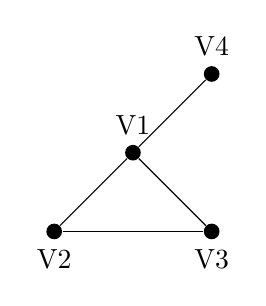
\begin{tikzpicture}
    % Nodes
    \node[circle, fill=black, inner sep=2pt, label=above:V1] (V1) at (1,1) {};
    \node[circle, fill=black, inner sep=2pt, label=below:V2] (V2) at (0,0) {};
    \node[circle, fill=black, inner sep=2pt, label=below:V3] (V3) at (2,0) {};
    \node[circle, fill=black, inner sep=2pt, label=above:V4] (V4) at (2,2) {};
  
    % Edges
    \draw (V1) -- (V2);
    \draw (V1) -- (V3);
    \draw (V1) -- (V4);
    \draw (V2) -- (V3);
  \end{tikzpicture}
%%%%%%%%%%%%%%%%%%%%%%%%%%%%%%%%%%%%
\section*{Exercise 15 4.2}  

Prove that every connected graph which is not itself a tree must have at last three different (although possibly isomorphic) spanning trees.


\vspace{0.5cm}
\noindent\textbf{Solution Draft:} 
\vspace{0.2cm}

\begin{enumerate}
    \item If a graph $G$ is connected but not a tree, then it must contain at least one cycle. 
    \item The minumum number of edges and verticies to contain a cycle is three.
    \item Therefore, we will always have at least three different spanning trees. This is because a triangle has 3 spanning trees which means anything higher than this will have three or more spanning trees.
\end{enumerate}
%%%%%%%%%%%%%%%%%%%%%%%%%%%%%%%%%%%%
\section*{Exercise 7b 4.3}  

Consider some classic polyhedrons.%
\begin{enumerate}
\item[b.] The traditional design of a soccer ball is in fact a (spherical projection of a) truncated icosahedron. This consists of 12 regular pentagons and 20 regular hexagons. No two pentagons are adjacent (so the edges of each pentagon are shared only by hexagons). How many vertices, edges, and faces does a truncated icosahedron have? Explain how you arrived at your answers. Bonus: draw the planar graph representation of the truncated icosahedron.%
\end{enumerate}

\vspace{0.5cm}
\noindent\textbf{Solution Draft:} 
\vspace{0.2cm}

\begin{itemize}
    \item  It has 12 regular pentagons and 20 regular hexagons, totaling 32 faces.
    \item  The has 60 vertices. Each original vertex from the icosahedron is replaced by a vertex of the added pentagon, where each vertex connects to three hexagons.
    \item  It has 90 edges. Each edge belongs to two faces, either between two hexagons or a hexagon and a pentagon.
\end{itemize}

Euler's formula is used to verify the correctness of our count, showing that for any convex polyhedron:
\[
V - E + F = 2
\]
\[
60 - 90 + 32 = 2
\]


%%%%%%%%%%%%%%%%%%%%%%%%%%%%%%%%%%%%
\section*{Exercise 9 4.3}  

Prove Euler's formula using induction on the number of \emph{vertices} in the graph.

\vspace{0.5cm}
\noindent\textbf{Solution Draft:} 
\vspace{0.2cm}

\textbf{Base Case}
The simpliest connected planar graph only has one vertex and no edges. The number of faces would be one (the outter face).
\begin{align*}
2 &= V-E+F \\
2 &= 1-0+1
\end{align*}

\textbf{Inductive Case}

We want to prove that the formula for a connected planar graph with $k+1$ vertices holds true.

When we add a vertex to a graph by an edge:

\begin{enumerate}
    \item $V$ increases by $1$
    \item $E$ also increases by $1$ as a new edge is created
    \item $F$ does not change.
\end{enumerate}

\begin{align*}
    2 &= (V + 1) - (E + 1) + F \\
    2 &= V +1 - E + 1 + F \\
    2 &= V - E + F + 1 - 1 \\
    2 &= V - E + F
    \end{align*}
We can see that Euler's formula does not change.
\vspace{1cm}

When we add a edge to a graph inside a face:

\begin{enumerate}
    \item $V$ does not increase.
    \item $E$ increases by $1$.
    \item $F$ increases by $1$ as an existing face is split in two.
\end{enumerate}

\begin{align*}
    2 &= V - (E + 1) + (F + 1) \\
    2 &= V - E - 1 + F + 1 \\
    2 &= V - E + F + 1 - 1 \\
    2 &= V - E + F
    \end{align*}
We can see that Euler's formula does not change.
%%%%%%%%%%%%%%%%%%%%%%%%%%%%%%%%%%%%

\section*{Exercise 6 4.4}  

Prove the chromatic number of any tree is two. Recall, a tree is a connected graph with no cycles.%

\begin{enumerate}[label= (\alph*)]
    \item Describe a procedure to color the tree below.
        \begin{center}
            \includegraphics[width=0.8\linewidth]{Capture-2024-04-16-195919.png} % Adjust the path and filename as necessary
        \end{center}
    \item The chromatic number of \(C_n\) is two when \(n\) is even. What goes wrong when \(n\) is odd?
    \item Prove that your procedure from part (a) always works for any tree.
    \item Now, prove using induction that every tree has chromatic number 2.
\end{enumerate}
    

\vspace{0.5cm}
\noindent\textbf{Solution Draft:} 
\vspace{0.2cm}

\begin{enumerate}
    \item Start at one point, go to the next and switch colors, every other point connected to that once recieves the first color. Since this graph is a tree you will only need to use two colors
    \item When $n$ is odd, you will end up with two adjacent verticies of the same color since the cycles does not close evenly.
    \item The algorithm stated above will work for all trees.
    \item 

    \textbf{Base Case}
    For a single vertex tree, the algorithm works since you will only need once color.

    \textbf{Inductive Case}
    Assume every tree with $k$ verticies has a chromatic number of two. Consider a tree with $k+1$ verticies. By removing a leaf, you have a tree with $k$ verticies. No matter how many leafs you remove or add, the chromatic number will never change since it will never create a cycle.
\end{enumerate}

%%%%%%%%%%%%%%%%%%%
\section*{Exercise 10 4.4}  

Find the chromatic number of the graph below and prove you are correct.

\begin{center}
    \includegraphics[width=0.8\linewidth]{Capture-2024-04-16-200146.png} % Adjust the path and filename as necessary
\end{center}


\vspace{0.5cm}
\noindent\textbf{Solution Draft:} 
\vspace{0.2cm}

The chromatic number of the graph below is 3. You cannot use less colors than 3.

\begin{center}
    \includegraphics[width=0.8\linewidth]{/Users/xander/Desktop/Screenshot 2024-04-16 at 20.10.49.png} % Adjust the path and filename as necessary
\end{center}


%%%%%%%%%%%%%%%%%%%%%%%%%%%%%%%%%%%%
\section*{Size of Infinite Sets Problem}  

Determine which of the following sets are countable and which are uncountable.
\begin{enumerate}
    \item[a.] $\{a, b, c\}$
    \item[b.] All odd numbers in $\mathbb{N}$
    \item[c.] $\mathbb{N}$
    \item[d.] $\mathbb{Z}$
    \item[e.] $\mathbb{R}$
\end{enumerate}

\vspace{0.5cm}
\noindent\textbf{Solution Draft:} 
\vspace{0.2cm}

\begin{enumerate}
    \item[a.] Countable 
    \item[b.] Countable
    \item[c.] Countable
    \item[d.] Countable
    \item[e.] Uncountable
\end{enumerate}

%%%%%%%%%%%%%%%%%%%%%%%%%%%%%%%%%%%%
\section*{Works cited}
Discrete Mathematics: An Open Introduction, 3rd edition by Oscar Levin.
\end{document}